% This is text associated with the open textbook "Open Electromagnetics"
% See immediately below for author, date
% This work is licensed under the Creative Commons Attribution-ShareAlike 4.0 International License. (CC BY-SA 4.0) 
% To view a copy of the license, visit http://creativecommons.org/licenses/by-sa/4.0/

%ORB TITLE Equivalent Circuit Model for Reception, Redux
%ORB AUTHOR 0        # S.W. Ellingson, Virginia Tech (ellingson@vt.edu)
%ORB DATE 20191212   # yyyymmdd
%ORB ABSTRACT 

\label{m0216_Equivalent_Circuit_Model_for_Reception_Redux} % <-- Must match name of this file and module directory name.  Don't mess with this!

Section~\ref{m0206_Equivalent_Circuit_Model_for_Reception} provides an informal derivation of an equivalent circuit model for a receiving antenna.
This model is shown in Figure~\ref{m0216_AntennaEquivCircuitReception}.
%
\begin{figure}[b!] % <--- "[b!]" for first figure in section *only*; delete for 2nd and subsequent figures
\begin{center}
\pdftooltip{{  % note double braces
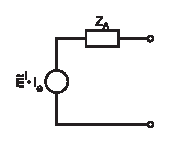
\includegraphics[width=1.5in]{modules/m0216_AntennaEquivCircuitReception.eps} 
% https://en.wikipedia.org/wiki/File:Sidelobes_en.svg
}}{Open circuit with source labeled capital E tilde superscript small i dot capital i sub small e. This is in series with capital Z sub capital A.}
\end{center}
\centerline{\scriptsize 
\copyright~\hyperref[m0216_AntennaEquivCircuitReception_Credit]{S.\ Lally} 
\href{https://creativecommons.org/licenses/by-sa/4.0/}{CC BY-SA 4.0}  
} % \centerline 
\caption{
\label{m0216_AntennaEquivCircuitReception}
Th\'{e}venin equivalent circuit model for an antenna in the presence of an incident electric field ${\bf E}^i$.
}
\end{figure}
%
The derivation of this model was informal and incomplete because the open-circuit potential ${\bf E}^i\cdot{\bf l}_e$ and source impedance $Z_A$ were not rigorously derived in that section.
While the open-circuit potential was derived in Section~\ref{m0215_Voltage_Induced_in_a_Dipole} (``Potential Induced in a Dipole''), the source impedance has not yet been addressed.
In this section, the source impedance is derived, which completes the formal derivation of the model.
Before reading this section, a review of Section~\ref{m0214_Reciprocity}  (``Reciprocity'') is recommended.

The starting point for a formal derivation is the two-port model shown in Figure~\ref{m0216_fTwoPort}.
%
\begin{figure} % <--- "[b!]" for first figure in section *only*; delete for 2nd and subsequent figures
\begin{center}
\pdftooltip{{  % note double braces
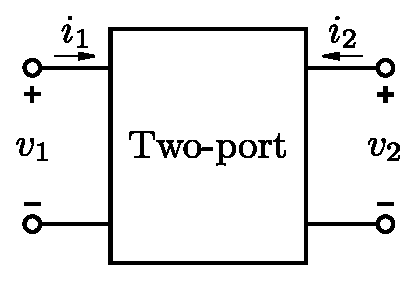
\includegraphics[width=1.5in]{modules/m0216_fTwoPort.eps} 
% https://commons.wikimedia.org/wiki/File:Two_Port_Circuit.svg
}}{Rectangle labeled Two-port with open terminals facing left and right. Left terminal small v subscript 1 and right terminal small v subscript 2 with upper limit positive. Current small i subscript 1 (left) and small i subscript 2 (right), both enter the device from the positive terminal.}
\end{center}
\centerline{\scriptsize 
\hyperref[m0216_fTwoPort_Credit]{Inductiveload}, 
public domain
(modified) 
} % \centerline 
\caption{
\label{m0216_fTwoPort}
Two-port system. 
}
\end{figure}
%
If the two-port is passive, linear, and time-invariant, then the potential $v_2$ is a linear function of potentials and currents present at ports~1 and 2.
Furthermore, $v_1$ must be proportional to $i_1$, and similarly $v_2$ must be proportional to $i_2$, so any pair of ``inputs'' consisting of either potentials or currents completely determines the two remaining potentials or currents.
Thus, we may write:
%
\begin{equation}
v_2 = Z_{21} i_1 + Z_{22} i_2
\label{m0216_ev2}
\end{equation} 
%
where $Z_{11}$ and $Z_{12}$ are, for the moment, simply constants of proportionality.
However, note that $Z_{11}$ and $Z_{12}$ have SI base units of $\Omega$, and so we refer to these quantities as impedances.
Similarly we may write:
%
\begin{equation}
v_1 = Z_{11} i_1 + Z_{12} i_2
\label{m0216_ev1}
\end{equation} 

We can develop expressions for $Z_{12}$ and $Z_{21}$ as follows.
First, note that $v_{1}=Z_{12}i_2$ when $i_1=0$.  
Therefore, we may define $Z_{12}$ as follows:
%
\begin{equation}
Z_{12} \triangleq \left.\frac{v_1}{i_2}\right|_{i_1=0}
\end{equation}
%
The simplest way to make $i_1=0$ (leaving $i_2$ as the sole ``input'') is to leave port~1 open-circuited.
In previous sections, we invoked special notation for these circumstances.
In particular, we defined
$\widetilde{I}_2^t$ as $i_2$ in phasor representation, with the superscript ``$t$'' (``transmitter'') indicating that this is the sole ``input''; and
$\widetilde{V}_1^r$ as $v_1$ in phasor representation, with the superscript ``$r$'' (``receiver'') signaling that port 1 is both open-circuited and the ``output.''
Applying this notation, we note:
%
\begin{equation}
Z_{12} = \frac{\widetilde{V}_1^r}{\widetilde{I}_2^t}
\label{m0216_eZ12}
\end{equation}

Similarly:
%
\begin{equation}
Z_{21} = \frac{\widetilde{V}_2^r}{\widetilde{I}_1^t}
\label{m0216_eZ21}
\end{equation}

In Section~\ref{m0214_Reciprocity} (``Reciprocity''), we established that a pair of antennas could be represented as a passive linear time-invariant two-port, with 
$v_1$ and $i_1$ representing the potential and current at the terminals of one antenna (``antenna~1''), and 
$v_2$ and $i_2$ representing the potential and current at the terminals of another antenna (``antenna~2'').
Therefore for any pair of antennas, quantities $Z_{11}$, $Z_{12}$, $Z_{22}$, and $Z_{21}$ can be identified that completely determine the relationship between the port potentials and currents.

We also established in Section~\ref{m0214_Reciprocity} that:
%
\begin{equation}
\widetilde{I}_1^t \widetilde{V}_1^r = \widetilde{I}_2^t \widetilde{V}_2^r
\label{m0216_eRIV}
\end{equation}
%
Therefore,
%
\begin{equation}
\frac{\widetilde{V}_1^r}{\widetilde{I}_2^t} = \frac{\widetilde{V}_2^r}{\widetilde{I}_1^t}
\label{m0216_eR1}
\end{equation}
%
Referring to Equations~\ref{m0216_eZ12} and \ref{m0216_eZ21}, we see that Equation~\ref{m0216_eR1} requires that:
%
\begin{equation}
Z_{12} = Z_{21}
\end{equation}
%
This is a key point.
Even though we derived this equality by open-circuiting ports one at a time, the equality must hold generally since Equations~\ref{m0216_ev2} and \ref{m0216_ev1} must apply -- with the same values of $Z_{12}$ and $Z_{21}$ -- regardless of the particular values of the port potentials and currents.

We are now ready to determine the Th\'{e}venin equivalent circuit for a receiving antenna.
Let port~1 correspond to the transmitting antenna; that is, $i_1$ is $\widetilde{I}_1^t$.
Let port~2 correspond to an open-circuited receiving antenna; thus, $i_2=0$ and $v_2$ is $\widetilde{V}_2^r$.
Now applying Equation~\ref{m0216_ev2}:
%
\begin{flalign}
v_2 &= Z_{21} i_1 + Z_{22} i_2 \nonumber \\
    &= \left(\widetilde{V}_2^r/\widetilde{I}_1^t\right) \widetilde{I}_1^t + Z_{22} \cdot 0 \nonumber \\
    &= \widetilde{V}_2^r
\end{flalign} 
%
We previously determined $\widetilde{V}_2^r$ from electromagnetic considerations to be (Section~\ref{m0215_Voltage_Induced_in_a_Dipole}): 
%
\begin{equation}
\widetilde{V}_2^r = \widetilde{\bf E}^i\cdot{\bf l}_e
\end{equation}
%
where $\widetilde{\bf E}^i$ is the field incident on the receiving antenna, and ${\bf l}_e$ is the vector effective length
\index{vector effective length}
as defined in Section~\ref{m0215_Voltage_Induced_in_a_Dipole}.
Thus, the voltage source in the Th\'{e}venin equivalent circuit for the receive antenna is simply $\widetilde{\bf E}^i\cdot{\bf l}_e$, as shown in Figure~\ref{m0216_AntennaEquivCircuitReception}.

The other component in the Th\'{e}venin equivalent circuit is the series impedance.
From basic circuit theory, this impedance is the ratio of $v_2$ when port~2 is open-circuited (i.e., $\widetilde{V}_2^r$) to $i_2$ when port~2 is short-circuited.
This value of $i_2$ can be obtained using Equation~\ref{m0216_ev2} with $v_2=0$:
%
\begin{equation}
0 = Z_{21} \widetilde{I}_1^t + Z_{22} i_2 
\end{equation}
%
Therefore:
 %
\begin{equation}
i_2 = - \frac{Z_{21}}{Z_{22}} \widetilde{I}_1^t  
\end{equation}
%
Now using Equation~\ref{m0216_eZ21} to eliminate $\widetilde{I}_1^t$, we obtain:
 %
\begin{equation}
i_2 = - \frac{\widetilde{V}_2^r}{Z_{22}} 
\end{equation}
%
Note that the reference direction for $i_2$ as defined in Figure~\ref{m0216_fTwoPort} is opposite the reference direction for short-circuit current.
That is, given the polarity of $v_2$ shown in Figure~\ref{m0216_fTwoPort}, the reference direction of current flow through a passive load attached to this port is from ``$+$'' to ``$-$'' through the load.
Therefore, the source impedance, calculated as the ratio of the open-circuit potential to the short circuit current, is:
%
\begin{equation}
\frac{\widetilde{V}_2^r}{+\widetilde{V}_2^r/Z_{22}} = Z_{22}
\end{equation}
%
We have found that the series impedance $Z_A$ in the Th\'{e}venin equivalent circuit is equal to $Z_{22}$ in the two-port model.
  
To determine $Z_{22}$, 
let us apply a current $i_2=\widetilde{I}_2^t$ to port~2 (i.e., antenna~2).
Equation~\ref{m0216_ev2} indicates that we should see:
%
\begin{equation}
v_2 = Z_{21} i_1 + Z_{22} \widetilde{I}_2^t
\end{equation}
%
Solving for $Z_{22}$:
%
\begin{equation}
Z_{22} = \frac{v_2}{\widetilde{I}_2^t} - Z_{21} \frac{i_1}{\widetilde{I}_2^t} 
\label{m0216_eZ22exact} 
\end{equation}
%
Note that the first term on the right is precisely the impedance of antenna~2 \emph{in transmission}. 
The second term in Equation~\ref{m0216_eZ22exact} describes a contribution to $Z_{22}$ from antenna~1.
However, our immediate interest is in the equivalent circuit for reception of an electric field $\widetilde{\bf E}^i$ in the absence of any other antenna.
We can have it both ways by imagining that $\widetilde{\bf E}^i$ is generated by antenna~1, but also that antenna~1 is far enough away to make $Z_{21}$ -- the factor that determines the effect of antenna~1 on antenna~2 -- negligible.  Then we see from Equation~\ref{m0216_eZ22exact} that $Z_{22}$ is the impedance of antenna~2 when transmitting.

\vspace{1in} %%% FORMATTING KLUDGE

Summarizing:  
%
%%%%%%%%%%%%%%%%%%%%%%%%%%%%%%%%%%%%%%%%%%%%%%%
%ORB HIGHLIGHT
\begin{mdframed}[backgroundcolor=yellow!20,nobreak=true] 
The Th\'{e}venin equivalent circuit for an antenna in the presence of an incident electric field $\widetilde{\bf E}^i$ is shown in Figure~\ref{m0216_AntennaEquivCircuitReception}.  The series impedance $Z_A$ in this model is equal to the impedance of the antenna in transmission.
\end{mdframed}
%%%%%%%%%%%%%%%%%%%%%%%%%%%%%%%%%%%%%%%%%%%%%%%

{\bf Mutual coupling.}
\index{mutual coupling}
This concludes the derivation, but raises a follow-up question:
What if antenna~2 is present and \emph{not} sufficiently far away that $Z_{21}$ can be assumed to be negligible?
In this case, we refer to antenna~1 and antenna~2 as being ``coupled,'' and refer to the effect of the presence of antenna~1 on antenna~2 as \emph{coupling}.
\index{coupling}
Often, this issue is referred to as \emph{mutual coupling}, since the coupling affects both antennas in a reciprocal fashion.
It is rare for coupling to be significant between antennas on opposite ends of a radio link.
This is apparent from common experience.  For example, changes to a receive antenna are not normally seen to affect the electric field incident at other locations.
However, coupling becomes important when the antenna system is a \emph{dense array}; i.e., multiple antennas separated by distances less than a few wavelengths.
It is common for coupling among the antennas in a dense array to be significant.
Such arrays can be analyzed using a generalized version of the theory presented in this section.

%%%%%%%%%%%%%%%%%%%%%

{\bf Additional Reading:}
\begin{itemize}
\item ``\href{https://en.wikipedia.org/wiki/Th%C3%A9venin%27s_theorem}{Th\'{e}venin's Theorem}'' on Wikipedia.
\end{itemize}

%%%%%%%%%%%%%%%%%%%%%%

